%\chapter{Movimiento en una Dimensi\'on}\label{ch:Movimiento1d}
%

\epigraph{...It seemed that this poor ignorant Monarch-as he called himself-was persuaded that the Straight Line which he called his Kingdom, and in which he passed his existence, constituted the whole of the world, and indeed the whole of Space. Not being able either to move or to see, save in his Straight Line, he had no conception of anything out of it...}{Edwin A. Abbott, \emph{Flatland: a Romance of Many Dimensions}}

A diferencia del personaje principal de la novela de Edwin A. Abbott, nosotros habitamos un universo con tres dimensiones espaciales (mas uno temporal). Sin embargo, muchas veces lo m\'as sencillo es empezar nuestro estudio de los fen\'omenos f\'isicos con el menor n\'umero de dimensiones, para as\'i luego ir agregando m\'as complejidad y generalidad a nuestros modelos.

Empezaremos, entonces, con el estudio de la \textbf{cinem\'atica}, el cual es una porci\'on de la Mec\'anica Cl\'asica que describe el movimiento de distintos objetos f\'isicos. Asumiremos, entonces, que la mayor\'ia de los objetos que estudiemos (si no es que todos) son \textbf{part\'iculas} o se comportan como \'estas. Es decir, que son objetos que tienen masa pero de tama\~no infinitesimal. Por ejemplo, podemos tratar a la Tierra como una part\'icula y modelar su movimiento alrededor del sol ya que el radio de la Tierra es mucho menor comparado al radio de la \'orbita que \'esta toma alrededor del Sol.

\section{Posici\'on, Velocidad y Rapidez}\label{sec:posvelrap2}

De la misma manera que tenemos un sistema de referencia para definir los est\'andares de medici\'on para comparar la longitud, masa y tiempo, tendremos un sistema de coordenadas que nos permita indicar la \textbf{posici\'on} de una part\'icula. Por lo tanto, decir que una part\'icula se encuentra a $\SI{5}{\meter}$ de distancia tiene sentido \'unicamente si decimos \emph{respecto a qu\'e}; en este caso, respecto a nosotros mismos.

T\'ipicamente denotamos con $O$ al \textbf{or\'igen} de \'este sistema de coordenadas. Por lo tanto, en el ejemplo anterior, nosotros ser\'iamos el or\'igen de nuestro eje de coordenadas. Estaremos utilizando las \emph{coordenadas cartesianas}, pero existen muchas otras m\'as (depender\'a de la simetr\'ia del problema que quieran atacar). De manera un poco arbitraria, en \'este sistema de coordenadas posicionamos a los n\'umeros positivos hacia la derecha del or\'igen, al 0 en el or\'igen, y a los negativos a la izquierda de \'este. V\'ease la Figura \ref{fig:cart2}.

\begin{figure}[ht]
\centering
  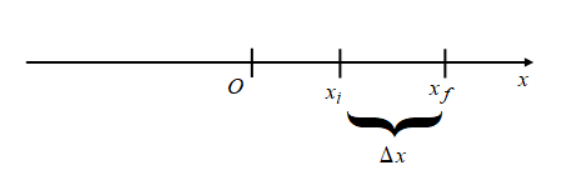
\includegraphics[width=0.8\textwidth]{lecture2/ejex.png}
\caption{Eje de coordenadas cartesianas en una dimensi\'on. Llamamos a la diferencia entre la posici\'on inicial $x_{i}$ y la final $x_{f}$ ell desplazamiento $\Delta x$. N\'otese que \'este puede ser positivo o negativo.}
\label{fig:cart2}
\end{figure}

Si tenemos, a lo largo de ciertos intervalos de tiempo, las mediciones de la posici\'on de un objeto, podemos calcular el desplazamiento de \'este. El \textbf{desplazamiento} de una part\'icula se define como su cambio en la posici\'on en un intervalo de tiempo. Es decir, que si nuestra part\'icula empieza en una posici\'on inicial $x_{i}$ y se mueve a una posici\'on final $x_{f}$, su desplazamiento estar\'a dado por:

\begin{equation}\label{eq:desplazamiento}
    \Delta x = x_{f} - x_{i}
\end{equation}

donde denotamos al desplazamiento por $\Delta x$. En general, utilizaremos a la letra griega $\Delta$ para denotar un cambio, ya sea en la posici\'on, tiempo, o cualquier otra cantidad f\'isica. N\'otese, entonces, que el desplazamiento puede ser positivo o negativo, todo depender\'a de las posiciones iniciales y finales de nuestra part\'icula (v\'ease la Figura \ref{fig:cart2}).

Es de notar el desplazamiento no es igual a la distancia recorrida por el veh\'iculo. En efecto, la \textbf{distancia} es la longitud total del camino tomado por cualquier part\'icula en un intervalo de tiempo definido (v\'ease la Figura \ref{fig:despl2}). Por lo tanto, la distancia \'unicamente puede ser cero o positiva, nunca negativa. Por lo tanto, llamamos a la distancia una \textbf{cantidad escalar} ya que solo tiene \emph{magnitud}, mientras que el desplazamiento es una \textbf{cantidad vectorial}, ya que tiene tanto \emph{magnitud} como \emph{direcci\'on}. \'Esta distinci\'on se har\'a m\'as notoria en el siguiente cap\'itulo.

\begin{figure}[ht]
\centering
  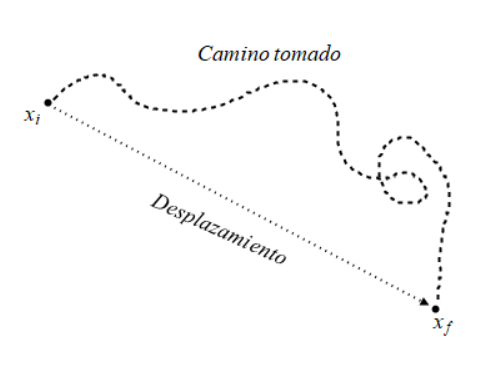
\includegraphics[width=0.8\textwidth]{lecture2/desplazamiento.PNG}
\caption{Desplazamiento entre dos puntos inicial y final, $x_{i}$ y $x_{f}$. N\'otese que la longitud del camino tomado ser\'a la distancia total recorrida $d$.}
\label{fig:despl2}
\end{figure}

Usualmente denotamos a la distancia por la letra $d$ y la escribimos de la siguiente manera (si no se siente c\'omodo a\'un con la notaci\'on, ignore la siguiente ecuaci\'on):

\begin{equation}\label{eq:distancia}
    d = \sum_{i=0}^{N}\lvert x(t_{i+1}) - x(t_{i}) \rvert = \sum_{i=1}^{N}\lvert \Delta x_{i} \rvert 
\end{equation}

Como un ejemplo sencillo para poder distinguir a la distancia y al desplazamiento, piense en su recorrido en un d\'ia normal: usted sale de su casa, hace su recorrido (se cual sea \'este) y al final, regresa a su casa. Su desplazamiento, entonces, al empezar y finalizar el d\'ia fue de cero, mas su distancia recorrida fue mayor a cero. 

\begin{ejemplo}\label{ej:carro2}
Analizemos el movimiento de un autom\'ovil que se mueve sobre el eje $x$. Las mediciones de su posici\'on las tendremos cada \SI{10}{\second}. Por lo tanto, tendremos la siguiente tabla de mediciones:

\begin{table}[ht]
\caption{Posici\'on del autom\'ovil en varios tiempos}
\begin{tabular}{l rrrr}
\toprule
\textbf{Posici\'on}  & \textbf{$t$ ($\si{\second}$)} & \textbf{$x$ ($\si{\meter}$)} & \textbf{$\Delta x$ ($\si{\meter}$)} & \textbf{$d$ ($\si{\meter}$)}\\
\midrule
$A$ & 0 & 30 & \-- & 0\\
$B$ & 10 & 52 & 22 & 22\\
$C$ & 20 & 38 & -14 & 36\\
$D$ & 30 & 0 & -38 & 74\\
$E$ & 40 & -37 & -37 & 111\\
$F$ & 50 & -53 & -16 & 127\\
\bottomrule
\end{tabular}
\label{table:carro1d2}
\end{table}

N\'otese que con s\'olo las primeras dos columnas podemos llenar las \'ultimas dos columnas de desplazamiento y distancia. Presentar la informaci\'on en forma de tabla es importante, pero el ser humano es muy visual, as\'i que proseguiremos a presentar la posici\'on del veh\'iculo en funci\'on del tiempo. V\'ease la Figura \ref{fig:posdist2}. A \'este tipo de gr\'aficas se les llama \emph{gr\'afica posici\'on-tiempo}.

\begin{figure}[ht]
    \centering
    \animategraphics[controls={play, step,stop},loop,width=0.8\textwidth]{1}{./gif/posdist/posdist-}{0}{3}
    \caption{Gr\'aficas de posici\'on del veh\'iculo y de la distancia recorrida. ?`Cu\'al es cu\'al? N\'otese que podemos generar mejores curvas que unan a los puntos, pero no necesariamente quiere decir que la posici\'on y la distancia se comporten de \'esta manera. Juegue con \'este usando Adobe Acrobat Reader.}
    \label{fig:posdist2}
\end{figure}

Es posible dibujar una curva que una todos nuestros puntos, pero a menos que sepamos exactamente c\'omo se mueve el veh\'iuclo, s\'olo ser\'ia un modelo de infinitos posibles. Por lo tanto, a\'un no podemos graficar con exactitud c\'omo se mueve el veh\'iculo, a menos que incrementemos nuestra frecuencia de muestreo (es decir, reduzcamos el intervalo de tiempo en el cual tomamos los datos).

\hfill $\square$
\end{ejemplo}

Otra forma de analizar los datos que tenemos es combinando las cantidades medidas de otra manera. N\'otese en la Tabla \ref{table:carro1d2} que en algunos tramos de la trayectoria, el veh\'iculo recorri\'o una mayor distancia que en otros.  La forma m\'as com\'un para comparar \'este tipo de movimiento es dividiendo el desplazamiento hecho, $\Delta x$, por el intervalo de tiempo durante el que ocure \'este desplazamiento, $\Delta t$. A \'esto se le llama \textbf{velocidad promedio} y se denota por $v_{x, \text{prom}}$, es decir:

\begin{equation}\label{eq:velprom2}
    v_{x, \text{prom}}\equiv \frac{\Delta x}{\Delta t}
\end{equation}

Debido a que el $\Delta t > 0$\footnote{Y a\'un no sabemos por qu\'e: \url{https://goo.gl/TtPYjZ}}, el signo de la velocidad promedio depender\'a entonces del signo del desplazamiento realizado. Por lo tanto, si la part\'icula se desplaza hacia la derecha, tendremos que $\Delta x >0$; si se desplaza hacia la izquierda, entonces $\Delta x < 0$ y si se queda quieto, entonces $\Delta x = 0$. Respectivamente, esto querr\'a decir que la velocidad promedio de la part\'icula ser\'a positiva ($v_{x, \text{prom}} > 0$), negativa ($v_{x, \text{prom}} < 0$) o igual a cero ($v_{x, \text{prom}} = 0$). N\'otese, entonces que esto implica que la velocidad ser\'a una \emph{cantidad vectorial}.

Las dimensiones de la velocidad promedio ser\'an $\si{\length/\time}$, o en el SI, $\si{\meter/\second}$. Podemos interpretar, en nuestra gr\'afica de la Figura \ref{fig:cart2}, a la velocidad promedio como la \textbf{pendiente de la l\'inea que une a dos puntos en nuestra trayectoria en nuestra gr\'afica posici\'on-tiempo}. 

Como \'ultima parte de \'esta secci\'on, definiremos un nuevo t\'ermino: la rapidez. En el d\'ia a d\'ia, es usual confundir los t\'erminos de velocidad con rapidez, pero en la F\'isica hay una gran distinci\'on. La \textbf{rapidez promedio} (una \emph{cantidad escalar}) se define como la distancia total viajada $d$ dividida por el tiempo total que se tom\'o en viajar dicha distancia, es decir:

\begin{equation}\label{eq:rapprom2}
    v_{\text{prom}}\equiv \frac{d}{\Delta t}
\end{equation}

Sus dimensiones tambi\'en ser\'an \si{\length/\time} y en el SI, \si{\meter/\second}. N\'otese, entonces, que como tratamos con una cantidad escalar, la rapidez promedio no tendr\'a signo, es decir, no tendr\'a direcci\'on: $v_{\text{prom}} \geq 0$. 

\begin{ejemplo}
Encuentre la velocidad y rapidez promedio del veh\'iculo del Ejemplo \ref{ej:carro2} entre los puntos $A$ y $F$.
\end{ejemplo}

\begin{solution*}

Nuestros puntos inicial y final ser\'an los puntos $A$ y $F$, por lo que:

\begin{equation*}
    \Delta x = x_{f}-x_{i}=x_{F} - x_{A} = \SI{-53}{\meter} - \SI{30}{\meter}=\SI{-83}{\meter}
\end{equation*}

El intervalo de tiempo durante este tramo del recorrido es:

\begin{equation*}
    \Delta t = t_{f}-t_{i}=t_{F} - t_{A} = \SI{50}{\second} - \SI{0}{\second}=\SI{50}{\second}
\end{equation*}

Por lo tanto, la velocidad promedio, usando la Ecuaci\'on \ref{eq:velprom2}, ser\'a:

\begin{equation*}
    v_{x, \text{prom}}= \frac{\Delta x}{\Delta t} = \frac{\SI{-83}{\meter}}{\SI{50}{\second}}=+\SI{1.7}{\meter/\second}
\end{equation*}

Para obtener la rapidez promedio, necesitaremos usar todos los otros puntos para calcular la distancia total recorrida por el veh\'iculo. De suerte, ya hemos calculado \'esto, por lo que $d=\SI{127}{\meter}$. Por lo tanto, la rapidez promedio ser\'a:

\begin{equation*}
    v_{\text{prom}}= \frac{d}{\Delta t} = \frac{\SI{127}{\meter}}{\SI{50}{\second}}=+\SI{2.5}{\meter/\second}
\end{equation*}

\hfill $\square$
\end{solution*}

\section{Velocidad y Rapidez Instant\'aneas}\label{sec:valrapinst2}

La velocidad y rapidez promedio no siempre son la mejor manera de analizar el movimiento de la part\'icula en cuesti\'on. En efecto, a veces deseamos conocer la rapidez o velocidad de una part\'icula \emph{en un instante}. Para \'este fin, Newton \href{https://www.youtube.com/watch?v=X_xR5Kes4Rs}{invent\'o} el C\'alculo, una poderosa herramienta que al d\'ia de hoy seguimos utilizando, inclusive para \href{https://towardsdatascience.com/gradient-descent-in-a-nutshell-eaf8c18212f0}{entrenar agentes de Inteligencia Artificial}. 

Previamente, discutimos acerca de la interpretaci\'on gr\'afica de la velocidad promedio, siendo \'esta la pendiente de la recta que une a dos puntos en la gr\'afica posici\'on-tiempo. Dicha recta se llama la \emph{l\'inea secante}. ?`Qu\'e pasar\'ia con el valor de \'esta pendiente si ambos puntos tienden a ser el mismo? V\'ease la Figura \ref{fig:secantder2}, donde tratamos de responder \'esta pregunta de manera gr\'afica.

\begin{figure}[ht]
    \centering
    \animategraphics[controls={play, step,stop},loop,width=\textwidth]{10}{./gif/tangent/tangent-}{0}{21}
    \caption{Las l\'ineas secantes y tangentes a una curva en unos puntos espec\'ificos. N\'otese que, al hacer que la distancia entre los dos puntos (rojo y azul) tiendan a cero, las pendientes de ambas l\'ineas tienden al mismo valor. Juegue con \'este usando Adobe Acrobat Reader.}
    \label{fig:secantder2}
\end{figure}

Por lo tanto, \textbf{la pendiente de la recta tangente a un punto en la curva de posici\'on de una part\'icula ser\'a su \emph{velocidad instant\'anea} en dicho punto}. Dicho de otra manera, empleando el lenguaje del C\'alculo, la velocidad instant\'anea, $v_{x}$ ser\'a la proporci\'on $\Delta x/\Delta t$ cuando $\Delta t$ tiende a cero, i.e.:

\begin{equation}\label{eq:deriv2}
    v_{x}\equiv \lim_{\Delta t\to0} \frac{\Delta x}{\Delta t}=\frac{dx(t)}{dt}
\end{equation}

La \'ultima igualdad es la notaci\'on de Leibniz y es la que m\'as utilizaremos. N\'otese que, ya que seguimos tratando con una pendiente a una curva, \'esta puede ser positiva, negativa o igual a cero, por lo que la velocidad instant\'anea seguir\'a siendo una cantidad vectorial. La \textbf{rapidez instant\'anea} ser\'a la magnitud de la velocidad instant\'anea, por lo que ser\'a una cantidad escalar. En la Tabla \ref{table:vel2} presentamos ciertos rangos de rapidez instant\'anea para saber los distintos rangos que podremos encontrar en el Universo.

\begin{table}[ht]
\caption{Rapidez de varios objetos observados}
\begin{tabular}{l r}
\toprule
           & \textbf{Rapidez (\si{\kilo\meter/\hour})} \\
\midrule
OMG Particle & $c-5.4\times10^{-15}$\\
Protones en LHC (7 TeV) & $1.079\times10^{9}$\\
S2 (orb. Sagitario $A^*$) &  $1.8\times10^{7}$ \\
PSR B2224+65 (pos. dejando la VL)  &  $5.8\times10^{6}$  \\
V\'ia L\'actea (rel. Fondo de Microondas) & $1.99\times10^6$\\
Andr\'omeda (acerc\'andose a nosotros) & $1.08\times10^6$\\
Sistema Solar alrededor de la V\'ia L\'actea & $7\times10^5$\\
Tierra alrededor del Sol & $1.07\times10^5$\\
Voyager 1 & $6.1\times10^4$\\
Rapidez de escape de la Tierra & $4.03\times10^4$\\
Estaci\'on Espacial Internacional & $2.77\times10^4$\\
Transbordador Espacial (STS) & $5.04\times10^3$\\
La Tierra (Punto en el Ecuador) & $1.67\times10^3$\\
Sonido en atm\'osfera est\'andar & $1.2\times10^3$\\
Airbus A380 & $9\times10^2$\\
Viento de un tornado grande & $468$\\
Formula Rossa (monta\~na rusa) & $240$\\
Usain Bolt (\SI{100}{\meter} en 2009) & $44.72$\\
Marcha promedio para un humano & $3.6\to5.4$\\
Crecimiento de bamb\'u & $5.0\times10^{-5}$\\
Ritmo promedio que se aleja la Luna  de la Tierra & $4.7\times10^{-9}$ \\
Deriva continental & $1\times10^{-9}\to1\times10^{-8}$\\
Ritmo de expansi\'on entre 2 puntos en el espacio a \SI{1}{\meter} & $7.8\times10^{-18}$\\
\bottomrule
\end{tabular}
\label{table:vel2}
\end{table}

De aqu\'i en adelante, utilizaremos a la palabra \emph{velocidad} para denotar a la velocidad instant\'anea y, de hablarse de la velocidad promedio, utilizaremos tal adjetivo.

\begin{ejemplo}
Una part\'icula se mueve a lo largo del eje $x$. Su posici\'on var\'ia con el tiempo de acuerdo a la expresi\'on $x=-4t+2t^2$\footnote{Lo correcto es escribir $x(t)=(-4.0\si{\meter/\second})t+(2.00\si{\meter/\second^2})t^{2.00}$, pero no est\'a mal ignorar las dimensiones de las constantes, siempre que tengan sentido desde un principio.}, donde $x$ est\'a en metros y $t$ en segundos. $a)$ Dibuje la gr\'afica posici\'on-tiempo de la part\'icula. $b)$ Calcule el desplazamiento de la part\'icula en los intervalos de tiempo de $t=0\si{\second}$ a $t=1\si{\second}$ y de $t=1\si{\second}$ a $t=3\si{\second}$. $c)$ Calcule la velocidad promedio durante estos dos intervalos de tiempo. $d)$ Encuentre la velocidad instant\'anea de la part\'icula en $t=2.5\si{\second}$.
\end{ejemplo}

\begin{solution*}
\begin{enumerate}[label=\alph*)]
    \item N\'otese que podemos escribir a la curva de la trayectoria como: $x=2t(t-2)$, por lo que la part\'icula cruzar\'a el eje $t$ cuando $t=0\si{\second}$ y  $t=2\si{\second}$. Como la curva es una par\'abola abierta hacia arriba, y por simetr\'ia, sabremos que el m\'inimo de la misma se encontrar\'a en el punto medio entre las intersecciones en el eje $t$, es decir: $x(1)=-4(1)+2(1)^2=-2\si{\meter}$. Con \'esto, podemos recrear la curva de la par\'abola:

\begin{figure}[ht]
\centering
  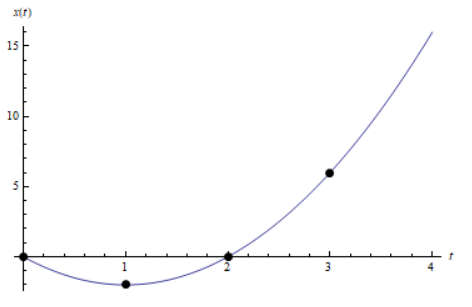
\includegraphics[width=\textwidth]{lecture2/plotparab.PNG}
\caption{Posici\'on de la part\'icula que estamos analizando en el ejercicio.}
\label{fig:plotparab2}
\end{figure}    

    \item Llamemos al punto $A$ al punto cuando $t=\SI{0}{\second}$; al punto $B$ al punto cuando $t=\SI{1}{\second}$; al punto $C$ al punto cuando $t=\SI{3}{\second}$. Entonces, tendremos que los desplazamientos son:
    
    \[ \Delta x_{A\to B} = x_{B} - x_{A} = (-4(1)+2(1)^2) - (-4(0)+2(0)^2) = -4+2=-2\si{\meter} \]
    y
    \[ \Delta x_{B\to C} = x_{C} - x_{B} = (-4(3)+2(3)^2) - (-4(1)+2(1)^2) = -12+18+4-2=+8\si{\meter} \]
    
    \item Tendremos que:
    
    \[ v_{x, \text{prom}}^{A\to B} = \frac{\Delta x_{A\to B}}{\Delta t_{A\to B}} = \frac{\SI{-2}{\meter}}{\SI{1}{\second}}=\SI{-2}{\meter/\second} \]
    y
    \[ v_{x, \text{prom}}^{B\to C} = \frac{\Delta x_{B\to C}}{\Delta t_{B\to C}} = \frac{\SI{8}{\meter}}{\SI{2}{\second}}=+\SI{4}{\meter/\second} \]
    
    \item Su libro de texto les dice, crudamente, que hay que medir la pendiente de la tangente en el punto dado. Si bien es factible, en este caso en espec\'ifico tienen a mano la curva exacta que toma la part\'icula. Por lo tanto, utilizaremos la Ecuaci\'on \ref{eq:deriv2}:
    
    \begin{equation*}
    \begin{split}
        v_{x}(t) &= \lim_{\Delta t\to0} \frac{\Delta x}{\Delta t} = \lim_{\Delta t\to0} \frac{x(t+\Delta t) - x(t)}{\Delta t}\\
        &=\lim_{\Delta t\to0}\frac{\left(-4(t+\Delta t)+2(t+\Delta t)^2\right) - \left(-4t+2t^2\right)}{\Delta t}\\
        &=\lim_{\Delta t\to0}\frac{\cancel{-4t}-4\Delta t\cancel{+2t^2}+4t\Delta t+2\Delta t^2\cancel{+4t}\cancel{-2t^2}}{\Delta t}\\
        &=\lim_{\Delta t\to0}\frac{-4\cancel{\Delta t}+4t\cancel{\Delta t}+2\Delta t^{\cancel{2}}}{\cancel{\Delta t}}\\
        &=\lim_{\Delta t\to0} \left( -4+4t+2\Delta t \right)\\
        &=-4+4t
    \end{split}
    \end{equation*}
    
    Por lo tanto, la velocidad instant\'anea en $t=\SI{2}{\second}$ ser\'a:
    
    \[ v_{x}(2.5\si{\second}) =  -4+4(2.5)=-4+10=+\SI{6}{\meter/\second}\]
    
    Pruebe medir la pendiente de la tangente de su libro de texto y comprobar que, en efecto, la pendiente es positiva y tiene valor 6.

\end{enumerate}

\hfill $\square$
\end{solution*}

\section{Modelo de An\'alisis: La part\'icula bajo velocidad constante}\label{sec:velcte2}

Cuando analizamos un carro, persona, estrella, o cualquier objeto, y reconocemos que se mueve con una velocidad constante, entonces las propiedades intr\'insicas de cada objeto no nos importan, ni nos afectar\'an en nuestros c\'alculos. \'Esto nos permitir\'a utilizar el modelo correcto, con el cual tendremos la lista adecuada de ecuaciones a utilizar \textbf{y NO viceversa}. Muchos cometen el error durante un examen, por ejemplo, de ver el listado de ecuaciones disponibles y utilizar alguna al azar. No s\'olo tendr\'an respuestas err\'oneas, sino que lo m\'as probable es que se compliquen m\'as de lo necesario.

Por lo tanto, reitero: el modelo de una \textbf{part\'icula que se mueve con velocidad constante} se puede aplicar a cualquier objeto que se puede modelar como una part\'icula que se mueve a velocidad constante, sin importar otros factores (tiene manos, es masivo, est\'a vivo, etc.).

Ya que la velocidad de la part\'icula es constante, su velocidad instant\'anea en cualquier instante durante un intervalo de tiempo ser\'a igual a la velocidad promedio durante dicho intervalo. Es decir, $v_{x}=v_{x,\text{prom}}$. 

\begin{equation*}
    v_{x}=\frac{\Delta x}{\Delta t}
\end{equation*}

Por lo tanto, usando la Ecuaci\'on \ref{eq:velprom2} y notando que en la pr\'actica utilizaremos a $t_{i}=\SI{0}{\second}$, llegamos a lo siguiente:

\begin{equation}\label{eq:velconst2}
    x_{f}=x_{i}+v_{x}t
\end{equation}

N\'otese que \'esta ecuaci\'on es la ecuaci\'on de una l\'inea recta con pendiente $v_{x}$ e intersecci\'on con el eje $x$ se da en $x_{i}$. Si se tiene la informaci\'on de que la part\'icula que se est\'a analizando se mueve a una velocidad constante, podemos r\'apidamente graficar su posici\'on como una l\'inea recta con las especificaciones previamente descritas.

\begin{ejercicio}
Una kinesi\'ologa estudia a un corredor que corre a lo largo de una l\'inea recta a un ritmo constante. Despu\'es de haber recorrido $4\si{\second}$, ella mide que el corredor se encuentra a $20\si{\meter}$ de cuando activ\'o el cron\'ometro. $a)$ ?`Cu\'al es la velocidad del corredor? $b)$ ?`Cu\'al es la posici\'on del corredor despu\'es de haber transcurrido $10\si{\second}$?
\end{ejercicio}

Una part\'icula que se mueve a \textbf{rapidez constante} no es lo mismo que una que se mueve a velocidad constante. En efecto, pueden haber casos en donde \'estos sean iguales, pero no siempre lo ser\'a debido a la naturaleza distinta de que una cantidad sea escalar y la otra vectorial. 

Continuando con la ecuaci\'on de la rapidez promedio, Ecuaci\'on \ref{eq:rapprom2}, denotaremos a la rapidez constante con $v$, por lo que:

\begin{equation}\label{eq:rapconst2}
    v = \frac{d}{\Delta t}
\end{equation}

\begin{ejemplo}
Imagine un \'aguila que circula los cielos tratando de localizar a su presa. Si se mueve a una rapidez constante de $\SI{5.00}{\meter/\second}$ y su trayectoria es circular con un radio de $\SI{10.0}{\meter}$, calcule entonces el intervalo de tiempo requerido para que el \'aguila complete un viaje alrededor del c\'irculo.
\end{ejemplo}

\begin{solution*}
Podemos utilizar la ecuaci\'on de rapidez constante, ya que sabemos que el \'aguila se mueve a rapidez constante. N\'otese que la distancia total recorrida es el per\'imetro de un c\'irculo. Por lo tanto, despejando a $\Delta t$ de la Ecuaci\'on \ref{eq:rapconst2}, tenemos que:

\[ \Delta t = \frac{d}{v} = \frac{2\pi r}{v} = \frac{2\pi(\SI{10.0}{\meter})}{\SI{5.00}{\meter/\second}} = \SI{4\pi}{\second}=\SI{12.6}{\second} \]

\hfill $\square$
\end{solution*}

\begin{ejercicio}
Calcule la rapidez promedio de la Tierra mientras \'esta gira alrededor del Sol. Utilize la Tabla \ref{table:distancias1} y note que la Tierra recorre \'esta distancia en 1 a\~no. ?`Cu\'anta distancia recorre la Tierra, entonces, en un d\'ia?
\end{ejercicio}

\section{Propuesta de modelo de an\'alisis para resolver problemas}

Su libro de texto propone unos pasos (modelo de an\'alisis) para poder llegar a la resoluci\'on de un problema a la hora de enfrentarse a \'este. Si bien cada quien tenga una forma distinta de enfrentarse y resolver problemas, quiz\'a alg\'un paso le sea \'util, sino es que todos.

\subsection{Conceptualizar}


\section{Aceleraci\'on}



\section{Diagramas de movimiento}



% \section{Modelo de An\'alisis: La part\'icula bajo aceleraci\'on constante}


